
Un bateau se trouve à une distance $d$ de la plage.

\begin{center}
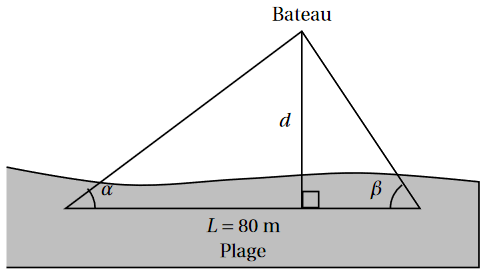
\includegraphics[scale=0.6]{TR-218-1.png} 
\end{center}

Supposons dans tout le problème que $\alpha = 45\degres, \beta = 65\degres$ et que $L = 80$ m.

\medskip

\begin{enumerate}
\item \textbf{Conjecturons la distance \boldmath$d$ \unboldmath à l'aide d'une construction}

\medskip

Mise au point par Thalès (600 avant JC), la méthode dite de TRIANGULATION
propose une solution pour estimer la distance $d$.
	\begin{enumerate}
		\item Faire un schéma à l'échelle 1/\np{1000} (1 cm pour 10 m).
		\item Conjecturer en mesurant sur le schéma la distance $d$ séparant le bateau de la côte.
	\end{enumerate}
\item \textbf{Déterminons la distance \boldmath$d$ \unboldmath par le calcul}

\begin{center}
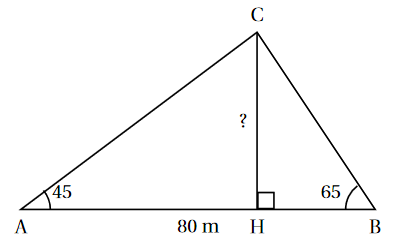
\includegraphics[scale=0.6]{TR-218-2.png} 
\end{center}

	\begin{enumerate}
		\item Expliquer pourquoi la mesure de l'angle $\widehat{\text{ACB}}$ est de $70$~\degres.
		\item Dans tout triangle ABC, on a la relation suivante appelée \og loi des sinus \fg :
  
\[\dfrac{\text{BC}}{\sin \widehat{\text{A}}} = \dfrac{\text{AC}}{\sin \widehat{\text{B}}} = \dfrac{\text{AB}}{\sin \widehat{\text{C}}}.\]

En utilisant cette formule, calculer la longueur BC. Arrondir au cm près.
		\item En déduire la longueur CH arrondie au cm près.
	\end{enumerate}
\end{enumerate}





